\documentclass[11pt]{standalone}

\usepackage{helvet}

\usepackage{ifthen}
\usepackage{tikz} 
\usetikzlibrary{shapes.misc}
\usetikzlibrary{arrows,arrows.meta}
\usetikzlibrary{calc,intersections, patterns, math}

\definecolor{pfeil}{RGB}{168,167,167}
\definecolor{petrol}{RGB}{0, 118, 136}
\definecolor{darkgoldenrod}{RGB}{184, 134, 11}
\colorlet{petrol-lighter}{petrol!40}
\colorlet{darkgoldenrod-lighter}{darkgoldenrod!40}

\begin{document}

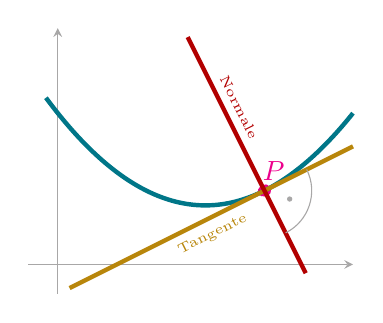
\begin{tikzpicture}[pfeil, scale=1.5]

    % \draw[thick, fill=petrol!20, draw=petrol-lighter, rounded corners=2ex, opacity=0.5] (0,0) rectangle ++ (1.5,3.5);
    % \draw[thick, fill=darkgoldenrod!20, draw=darkgoldenrod-lighter, rounded corners=2ex, opacity=0.5] (5,0) rectangle ++ (1.5,3.5);

    \draw[-stealth] (-0.25,0) -- (2.5,0);
    \draw[-stealth] (0,-0.25) -- (0,2);

    \draw[dashed, magenta, fill] (1.75,0.625) circle (0.05) node[above] {$\ \ P$};

    \draw[ultra thick,domain=-0.1:2.5, smooth, samples=50, petrol] plot(\x,{0.5*(\x-1.25)^2+0.5});

    \draw[ultra thick,domain=0.1:2.5, smooth, samples=50, darkgoldenrod] plot(\x,{0.5*\x-0.25});

    \draw[ultra thick,domain=1.1:2.1, smooth, samples=50, red!70!black] plot(\x,{-2*\x+4.125});
    
    \draw[] (1.75,0.625) ++ (26.56:0.4) arc (26.56:-63.43:0.4);
    \draw[fill] (1.75,0.625) ++(-18.43:0.225) circle (0.0175);

    \path (0.75,0.125) -- node[sloped, darkgoldenrod, below] {\tiny Tangente} (1.75,0.625);
    \path (1.1,1.925) -- node[sloped, red!70!black, above] {\tiny Normale} (1.75,0.625);
    

\end{tikzpicture}

\end{document}
